%\clearpage
\section{Webclient (CH)}
\label{section_webclient}
Der Webclient ist die Schnittstelle zwischen Nutzer und Anwendung. Nach Aufruf der Applikation wird der Nutzer aufgefordert seine Session-ID einzugeben. Ist diese gültig, gelangt er in seinen persönlichen Bereich. Dort wird er mit seinem Namen begrüßt und kann die Bilder aus seiner Fotosession betrachten. 

Die einzelnen Bilder werden zunächst zur Übersicht in einer Galerie mit quadratischen Thumbnails angezeigt. Durch Klick auf ein Thumbnail wird das entsprechende Bild vergrößert bzw. das Orginal-Bild angezeigt. Hierbei bietet die Galerie vier verschiedene Ansichtsmöglichkeiten. Auf Smartphones fällt die Auswahlmöglichkeit weg und die Bilder werden initial in der Borderless / Fullscreen Ansicht Dargestellt. 

\begin{itemize}
	\item Lightbox
	\item Borderless
	\item Lightbox / Fullscreen
	\item Borderless / Fullscreen
\end{itemize}

\begin{figure}[h]
	\centering
	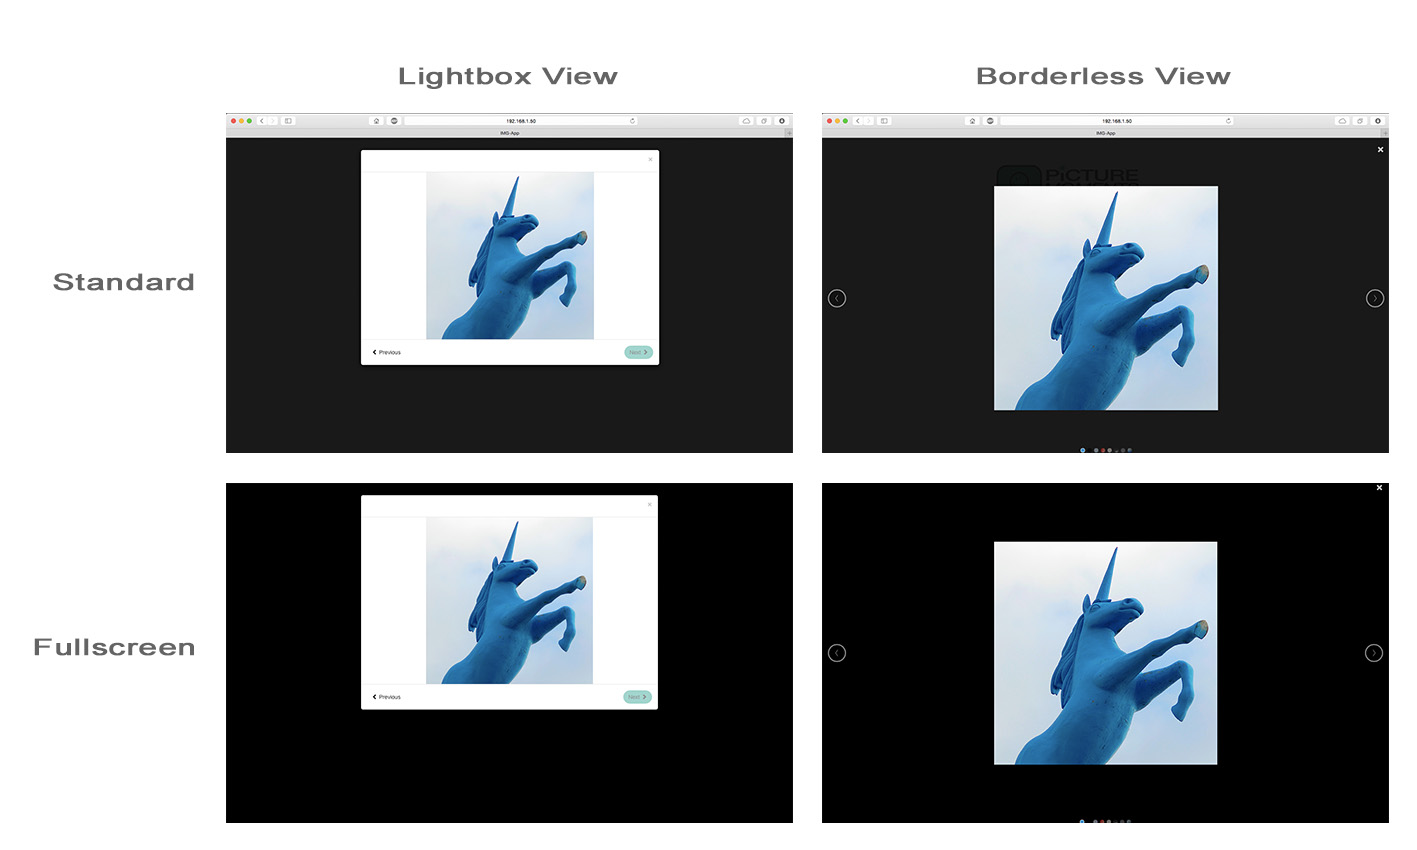
\includegraphics[width=14cm]{bilder/gallery_view}
	\caption{Galerie Ansichten}
	\label{fig_galerie_ansichten}
\end{figure}

In der Galerieansicht lässt sich jeweils zu dem nächsten oder vorherigen Bild via Button oder Pfeiltasten in Desktop Borwsern oder via Touch-Slide auf mobilen Endgeräten navigieren. 

\subsection{Schnittstellen}
Der Webclient hält folgende Schnittstellen bereit:

\begin{table}[h]
	\begin{center}
		\begin{tabularx}{\textwidth}{|c|l|X|}
			\hline
			\textbf{Methode} & \textbf{Pfad} & \textbf{Funktion}\\
			\hline
			GET & / & ruft die Datei index.html auf und bewirkt den Start der Anwendung \\
			\hline
			GET & /api/sessions/:id & ruft die Session mit gegebenen ID auf \\
			\hline
			GET & /api/thumbnails/:id & ruft ein Thumbnail des Bildes mit gegebenen ID ab \\
			\hline
			GET & /api/images/:id & ruft ein Bild mit gegebenen ID ab \\
			\hline
		\end{tabularx}
		\caption{Die zu realisierende Schnittstelle}
		\label{tab_api_routes}
	\end{center}
\end{table}

Mit der Eingabe der URL wird zunächst ein GET Request an den Webserver gestellt, der Webserver gib daraufhin die \textit{index.html} zurück.

Die weitere Kommunikation zwischen Client und Webserver verläuft über die im Webclient integrierte AJAX-Engine. Der Client stellt einen GET Request und bekommt die entsprechende Antwort in Form eines JSON Strings oder als Binärdaten zurück (Siehe Dazu auch Kapitel 3.1 und Abbildung 3)

\subsection{Realisierung}
Der Webclient basiert auf einer Single-Page Anwendung und wurde mittels der Grundelemente HTML (\textit{index.html}), CSS (\textit{style.css}), JavaScript (\textit{app.js}) implementiert. 

Neben diesen drei Elementen wurde zur Realisierung der Website das Framework Bootstrap und die JavaScript Bibliothek jQuery genutzt. Außerdem wurde zur Erstellung der Galerie auf die Bootstarp Image Gallery blueimp  zurückgegriffen.

Entsprechende Codezeilen des Bootstrap Stylesheets werden durch das Stylesheet \textit{style.css}, was individuelle Designvorgaben enthält, überschrieben. 

Die \textit{index.html} gibt die Struktur der Web-Anwendung vor. Sie beinhaltet das Logo, ein Jumbotron als Textfeld, das Formular zur Eingabe der Session ID und die entsprechenden Button.  Die Darstellung der Seite wird durch die \textit{app.js} gesteuert. Die Elemente werden je nach Bedarf ein- oder ausgeblendet. Dialogtexte sowie die Galerie werden dynamisch erzeugt aus der \textit{app.js} erzeugt. 

Des Weiteren stellt die \textit{app.js} die Funktion requestSession zur AJAX Kommunikation zwischen Webclient und Webserver bereit.

\begin{figure}[h]
	\begin{lstlisting}[caption={Auszug aus app.js}, label=list_client]
	function requestSession(evt) {
	
	var id = $('#inputSessionId').val();
	if (id !== '') {
	var jqxhr = $.ajax('/api/sessions/' + id)
	.done(function() {
	//alert('done');
	})
	.success(function(data, textStatus) {
	appendSessionView(data);
	})
	.fail(function(err) {
	$('#greeterHeading').css({"color": "#C1121C"}).html('Die eingegebene Session ID ist nicht vergeben. ' +
	'Bitte kontrolliere Deine Eingabe oder versuche es zu einem späteren Zeitpunkt noch einmal.');
	})
	.always(function() {
	//alert( "complete" );
	});
	} else {
	$('#greeterHeading').css({"color": "#C1121C"}).html('Es wurde keine Eingabe getätigt. ' +
	'Bitte gib Deine Session-ID ein.');
	}
	}
	\end{lstlisting}
\end{figure}

Der Client ruft hierbei Daten vom Webserver, die dort unter einer bestimmten Session ID gespeichert sind, ab. Bei einer ungültigen ID sendet der Webserver den Fehlercode 404 zurück an den Webclient und der Fail-Zweig der If-Abfrage wird ausgeführt. Bei einer gültigen Session ID wird der Success-Zweig ausgeführt und die Daten vom Webserver an die Funktion appendSessionView übergeben.

In der Funktion appendSessionView werden die Daten vom Webserver verarbeitet und dynamisch in die \textit{index.html} übergeben.

\begin{figure}[h]
	\begin{lstlisting}[caption={Auszug aus app.js}, label=list_client]
	var imagesHTML = '';
	sessionData.images.forEach(function(image) {
	
	var link = '<div class="col-xs-6 col-sm-5 col-md-4 col-lg-3"><a id="thumbnail" href="/api/images/' + image + '" class="thumbnail" data-gallery>';
	link += '<img src="/api/thumbnails/'
	+ image + '" class="img-responsive" width="" height="" alt="' + image + '" /></a>';
	
	link += '</div>';
	imagesHTML += link;
	
	});
	\end{lstlisting}
\end{figure}

Für jedes Bild wird hier in HTML-Syntax eine Div-Box mit den entsprechenden Attributen erstellt. 

\begin{figure}[h]
	\begin{lstlisting}[caption={Auszug aus app.js}, label=list_client]
	var name = sessionData.client.firstname + ' '
	+ sessionData.client.lastname;
	
	$('#greeterHeading').css({"color": "#8D9091"}).html('Hallo ' + name + '!<br/> Die Bilder Deiner Session liegen hier bereit. ' +
	'Du kannst Dich durch alle Bilder durchklicken und sie online betrachten. Viel Spass!');
	\end{lstlisting}
\end{figure}


Auch der Name wird aus den JSON Daten des Servers hier verarbeitet und mit weiterem Text an die index.html übergeben. 

Die Anwendung soll sowohl für Mobile- als auch für Desktopdevices geeignet sein. Daher soll es einige Unterschiede in der Darstellung das jeweilige Device geben. Beispielweise die eingangs erwähnte Darstellung der Bilder (initiale Ansicht in der Lightbox bei Desktop-Browsern mit der Option diese zu verändern und die Borderless/Fullscreen Ansicht für mobile Endgeräte). 

Die Unterscheidung der Geräte wird durch Funktionen, die die entsprechenden Geräte erkennen und an die Variable isMobile zurück geben. Durch eine If-Abfrage wird die Darstellung der Website für das entsprechende Device angepasst.

\begin{figure}[h]
	\begin{lstlisting}[caption={Auszug aus app.js}, label=list_client]
	// Variable to detect mobile devices
	var isMobile = {
	Android: function() {
	return navigator.userAgent.match(/Android/i);
	},
	BlackBerry: function() {
	return navigator.userAgent.match(/BlackBerry/i);
	},
	iOS: function() {
	return navigator.userAgent.match(/iPhone|iPad|iPod/i);
	},
	Opera: function() {
	return navigator.userAgent.match(/Opera Mini/i);
	},
	Windows: function() {
	return navigator.userAgent.match(/IEMobile/i);
	},
	any: function() {
	return (isMobile.Android() || isMobile.BlackBerry() || isMobile.iOS() || isMobile.Opera() || isMobile.Windows());
	}
	};
	
	// Gallery view for mobile and desktop devices
	if(isMobile.any()) {
	// Fullscreen and borderless gallery view for mobile devices
	$('#borderless-checkbox').prop('checked', function () {
	var borderless = $(this).is(':checked');
	$('#blueimp-gallery').data('useBootstrapModal', !borderless);
	$('#blueimp-gallery').toggleClass('blueimp-gallery-controls', borderless);
	});
	
	$('#fullscreen-checkbox').prop('checked', function () {
	$('#blueimp-gallery').data('fullScreen', $(this).is(':checked'));
	});
	
	}else {
	
	// Initial Lightbox view for desktop devices
	$('#borderless-checkbox').on('change', function () {
	var borderless = $(this).is(':checked');
	$('#blueimp-gallery').data('useBootstrapModal', !borderless);
	$('#blueimp-gallery').toggleClass('blueimp-gallery-controls', borderless);
	});
	
	$('#fullscreen-checkbox').on('change', function () {
	$('#blueimp-gallery').data('fullScreen', $(this).is(':checked'));
	});
	
	}
	
	\end{lstlisting}
\end{figure}

In diesem Beispiel wird die Ansichtsart der Bilder für die entsprechenden Devices 
festgelegt. Im ersten If-Zweig, welchher bei der Nutzung mobiler Geräte aufgerufen 
wird, werden durch prop() die Checkboxen, welche zur Auswahl der Darstellung 
dienen, initial als checkt gesetzt und somit die Darstellung auf Borderless/Fullscreen 
gesetzt.